\chapter{Real-Time Software and its testing}
\label{chap:rt}
\section{Real-Time Software}
Donald Gillies defined a real-time software as a system: \textit{"[...] in which the correctness of the computations not only depends upon the logical correctness of the computation but also upon the time at which the result is produced. If the timing constraints of the system are not met, system failure is said to have occurred."} While Robert L. Glass\cite{RealTimeTesting} defines this term as: \textit{"[...] a software that drives a computer which interacts with functioning external devices or objects. It is called real-time because the software actions control activities that are occurring in an ongoing process".} 

Within this research, we will define  Real-Time software as a combination of this to definitions and covers both logical and time correctness as well as an interaction with external systems controlled by the ongoing process. \textbf{Real-Time Software} \textit{is a type of software in which correctness of computations based on both internal and external inputs and/or outputs is valid if and only if the result of computation is logically correct and was obtained within the specified period of time.}

The Web-Banking engine of figo GmbH matches this definition due to the following facts. First, it performs communication with external systems (API customers input and Web Banking HTML pages). Next, its result depends on time restrictions (if child process responsible for script execution was not finished within 1200 seconds, and with each task performed within 0.5 seconds it is considered to be the failure) as well as logical correctness depended on the ability of the script to perform necessary actions for a fulfillment of a requested task.

%Within the scope of this research under Real-Time software we will mean the software that interact with external systems and its correctness depends on logical correctness of execution result as well as result production time.

%Not only do the programmers have to look at black/white box testing but also the timing of the data \& the parallelism of the projects. In lots of situations testing data for real-time technique may raise errors when the technique is in four state but to in others.\cite{strategicRT}

%"During the development of a real-time application, a testing step is necessary to check the conformity of the implementation in accordance with its specification. "\cite{trts}

%In general the special characteristic of real-time systems makes them a main challenge when it comes to testing. The time-dependent type of real-time applications adds a new difficult element to testing.

\section{Testing Real-Time software}
Tsai, Fang and Bi\cite{rtSandD} state that testing and debugging of real-time software are very difficult because of timing constraints and non-deterministic execution behavior. In a real-time system, the processes receive inputs from the real world processes as a result of asynchronous interrupts and it is almost impossible to precisely predict the exact program execution points at which the inputs will be supplied to the system. Consequently, the system may not exhibit the same behavior upon repeated execution of the program. In addition, in a real-time system, the pace of an execution of processes is determined not only by an internal criteria but also by real world processes and their timing constraints. 

The general testing and debugging strategy (Fig. \ref{fig:GeneralTestingAndDebugging}) described by Tsai, Fang and Bi \cite{rtSandD} consists of four steps.
At the \textit{first} step, a set of events which can be used to represent the program's execution behavior at a specific abstraction level and the event key values which describe these events are identified. 
At the \textit{second} step, the execution data, containing the event key values identified in the first step, is collected using the real-time monitoring system. 
The first and second steps constitute the monitoring phase. After the data is collected, at the \textit{third} step, the collected data is processed in an off-line mode to construct logical views to represent the program's execution behavior.
At the \textit{fourth} step, analysis algorithms will be employed to identify fault units and report them to the user. 
Finally, the user can use this report to decide next monitoring and debugging cycle for a lower level abstraction.
In this paper, the provided strategy is applied for each individual test.

\begin{figure}[ht]
	\centering
	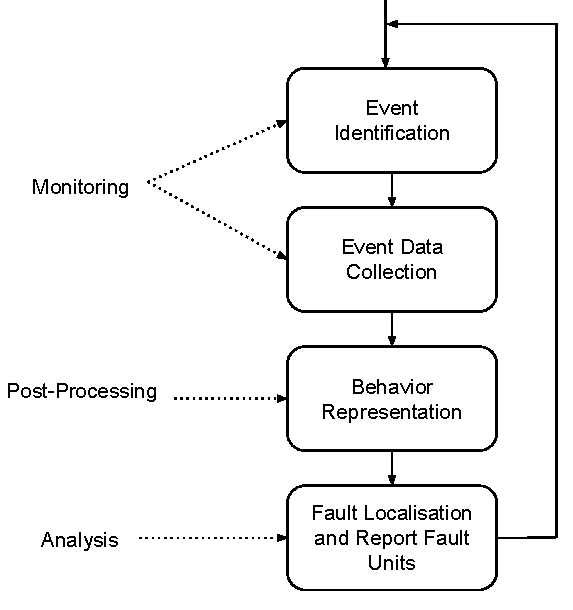
\includegraphics[width=0.7\linewidth]{grafiken/GeneralTestingAndDebugging}
	\label{fig:GeneralTestingAndDebugging}
	\caption{General Testing and Debugging Strategy\cite{rtSandD}}
\end{figure}

\section{Web scraping}
\label{sec:scraping}
Web scraping is a method for extracting information from web pages\cite{wikiScraping}. This technique is useful when you want to do real-time, price and product comparisons, archive web pages, or acquire data sets that you want to evaluate or filter\cite{conScrap}.

Web scraping works via interaction with Document Object Model (DOM) of the web page it is a useful technique for real-time data extraction from human readable web-pages. W3Council defines DOM\cite{w3cDOM} as "... a platform- and language-neutral interface that will allow programs and scripts to dynamically access and update the content, structure and style of documents." 

\subsection{Web scraping tools}

\paragraph{PhantomJS}\cite{phantom} \url{http://www.phantomjs.org} is a headless WebKit scriptable with JavaScript. 

\textbf{Use Cases:}
\begin{itemize}
	\item Headless web testing (without the browser).
	\item Page automation. Access and manipulate web pages with the standard DOM API, or with usual libraries like jQuery.
	\item Screen capture. Programmatically capture web contents, including CSS, SVG and Canvas.
	\item Network monitoring. Automate performance analysis, track page loading and export as standard HAR format.
\end{itemize}

\textbf{Features:}
\begin{itemize}
	\item Multiplatform, available on major operating systems: Windows, Mac OS X, Linux, and other Unices.
	\item Native implementation of web standards: DOM, CSS, JavaScript, Canvas, and SVG.
	\item Pure headless.
\end{itemize}

\paragraph{CasperJS} is an open source navigation scripting \& testing utility written in javascript for the headless browsing. It eases the process of defining a full navigation scenario and provides useful high-level functions, methods \& syntactic sugar for doing common tasks for interaction with DOM of the web page\cite{casperjs}:
\begin{itemize}
	\item defining \& ordering browsing navigation steps
	\item filling \& submitting forms
	\item clicking \& following links
	\item capturing screenshots of a page (or part of it)
	\item testing remote DOM
	\item logging events
	\item downloading resources, including binary ones
	\item writing functional test suites, saving results as JUnit XML
	\item scraping Web contents
\end{itemize}

The use of this tools gives an ability for figo GmbH to pragmatically imitate user behavior on a web page. Which includes filling login forms, filing forms for retrieving service information and perform other business activity available via a service web site. CasperJS instantiates a web-page or its part defined as a tree of DOM selectors.  Page content includes both HTML and javascript/jQuery code from the web-page addressed with provided URL. Instantiated page or its part is stored in memory and can be accessed for further manipulation by CasperJS methods as any other object instance.